%%%%%%%%%%%%%%%%%%%%%%%%%%%%%%%%%%%%%%%%%%%%%%%%%%%%%%%%%%%%%%%%%%%%%%%%%%%

\documentclass{standalone}

\usepackage{mathptmx}
\usepackage{tikz}
\usetikzlibrary{decorations.fractals}
\usetikzlibrary{external}
\tikzexternalize{koch-snowflake-2-area}

%% We default to Times.
\renewcommand{\rmdefault}{ptm}
\renewcommand{\ttdefault}{pcr}
%% Enable Times/Palatino main text font.
\normalfont\selectfont

%% The second iteration of the Koch snowflake.
\newcommand{\secondIteration}{%%
  %% The shaded shape.
  \draw[greyStyle] decorate{%%
      (origin) -- ++(\degree:\length) -- ++(-\degree:\length) -- cycle%%
    }
    -- cycle;
  %% Draw the second iteration.
  \draw[lineStyle] decorate{%%
    decorate{%%
      (origin) -- ++(\degree:\length) -- ++(-\degree:\length) -- cycle%%
    }%%
  }
  -- cycle;
}

%%%%%%%%%%%%%%%%%%%%%%%%%%%%%%%%%%%%%%%%%%%%%%%%%%%%%%%%%%%%%%%%%%%%%%%%%%%
%% The second iteration of the Koch snowflake.
%%%%%%%%%%%%%%%%%%%%%%%%%%%%%%%%%%%%%%%%%%%%%%%%%%%%%%%%%%%%%%%%%%%%%%%%%%%

\begin{document}

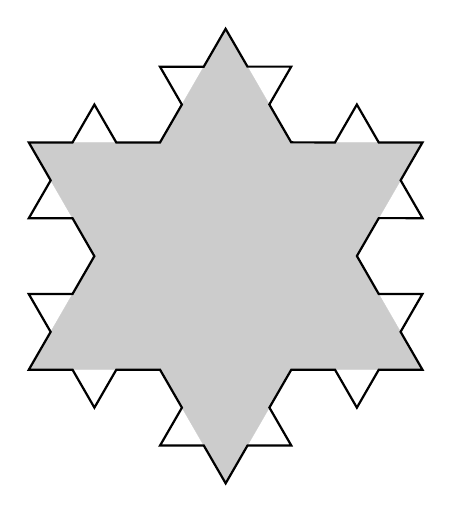
\begin{tikzpicture}[%%
  decoration=Koch snowflake,%%
  greyStyle/.style={-,ultra thin,fill=gray!40,gray!40},%%
  lineStyle/.style={-,thick}%%
]
%%
%%
\pgfmathsetmacro{\degree}{60}  %% Value of each internal angle.
\pgfmathsetmacro{\length}{5}   %% Length of each side of triangle.
\pgfmathsetmacro{\xlow}{0}
\pgfmathsetmacro{\ylow}{\xlow}
\coordinate (origin) at (\xlow,\ylow);
%%
%%
%% The second iteration of the Koch snowflake.
\secondIteration
\end{tikzpicture}

\end{document}
